\documentclass[ignorenonframetext,12pt,t]{beamer}
\setbeamertemplate{caption}[numbered]
\setbeamertemplate{caption label separator}{: }
\setbeamercolor{caption name}{fg=normal text.fg}
\beamertemplatenavigationsymbolsempty
\usepackage{lmodern}
\usepackage{amssymb,amsmath}
\usepackage{ifxetex,ifluatex}
\usepackage{fixltx2e} % provides \textsubscript
\usepackage{multicol}
\usepackage{multirow}
\usepackage{tabularx}
\newcolumntype{C}{>{\centering\arraybackslash}X}

\ifnum 0\ifxetex 1\fi\ifluatex 1\fi=0 % if pdftex
  \usepackage[T1]{fontenc}
  \usepackage[utf8]{inputenc}
\else % if luatex or xelatex
  \ifxetex
    \usepackage{mathspec}
  \else
    \usepackage{fontspec}
  \fi
  \defaultfontfeatures{Ligatures=TeX,Scale=MatchLowercase}
\fi
\usetheme[]{Honefoss}
% use upquote if available, for straight quotes in verbatim environments
\IfFileExists{upquote.sty}{\usepackage{upquote}}{}
% use microtype if available
\IfFileExists{microtype.sty}{%
\usepackage{microtype}
\UseMicrotypeSet[protrusion]{basicmath} % disable protrusion for tt fonts
}{}
\newif\ifbibliography
\hypersetup{
            pdftitle={Where - A New Software for Geodetic Analysis},
            pdfauthor={Geir Arne Hjelle; Ann-Silje Kirkvik; Michael Dähnn; Ingrid Fausk},
            pdfborder={0 0 0},
            breaklinks=true}
\urlstyle{same}  % don't use monospace font for urls

% Prevent slide breaks in the middle of a paragraph:
\widowpenalties 1 10000
\raggedbottom

\AtBeginPart{
  \let\insertpartnumber\relax
  \let\partname\relax
  \frame{\partpage}
}
\AtBeginSection{
  \ifbibliography
  \else
    \let\insertsectionnumber\relax
    \let\sectionname\relax
    \frame{\sectionpage}
  \fi
}
\AtBeginSubsection{
  \let\insertsubsectionnumber\relax
  \let\subsectionname\relax
  \frame{\subsectionpage}
}

\setlength{\parindent}{0pt}
\setlength{\parskip}{6pt plus 2pt minus 1pt}
\setlength{\emergencystretch}{3em}  % prevent overfull lines
\providecommand{\tightlist}{%
  \setlength{\itemsep}{0pt}\setlength{\parskip}{0pt}}
\setcounter{secnumdepth}{0}

%\title{Where -- A New Software for Geodetic Analysis}
\title{Where}
\subtitle{A New Software for Geodetic Analysis}
\author{Geir~Arne~Hjelle \and Ann-Silje~Kirkvik \and Michael~Dähnn \and Ingrid~Fausk}
\date{REFAG --- July 20, 2018\\}
\titlegraphic{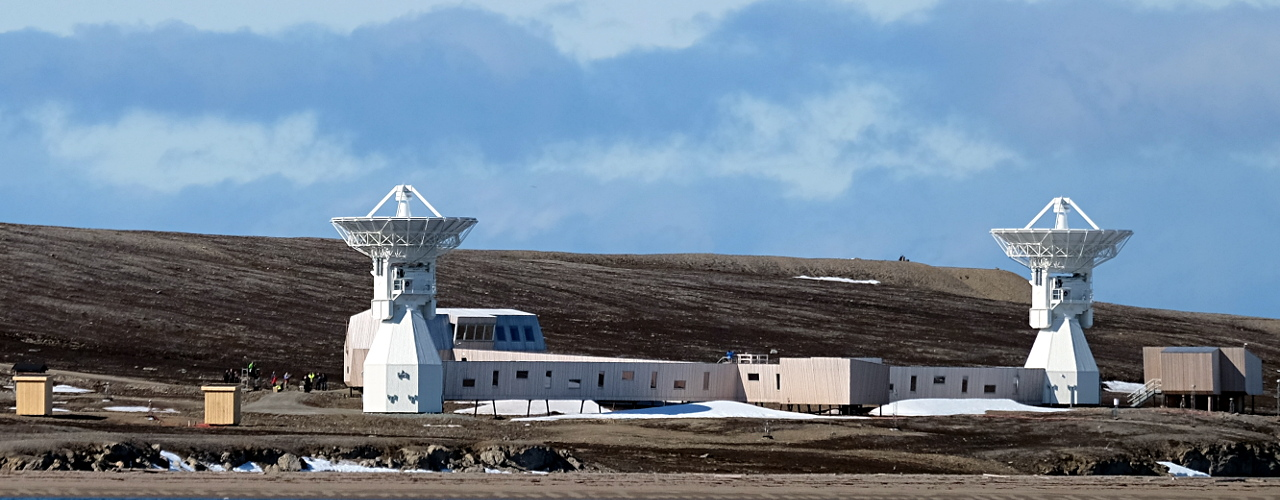
\includegraphics[width=\paperwidth]{figure/brandal}}

\begin{document}
\frame{\titlepage}


\begin{frame}[c]{Demo}
  \includegraphics[width=0.8\paperwidth]<1>{figure/where_demo01}
  \includegraphics[width=0.8\paperwidth]<2>{figure/where_demo02}
  \includegraphics[width=0.8\paperwidth]<3>{figure/where_demo03}
  \includegraphics[width=0.8\paperwidth]<4>{figure/where_demo04}
  \includegraphics[width=0.8\paperwidth]<5>{figure/where_demo05}
  \includegraphics[width=0.8\paperwidth]<6>{figure/where_demo06}
  \includegraphics[width=0.8\paperwidth]<7>{figure/where_demo07}
  \includegraphics[width=0.8\paperwidth]<8>{figure/where_demo08}
  \includegraphics[width=0.8\paperwidth]<9>{figure/where_demo09}
  \includegraphics[width=0.8\paperwidth]<10>{figure/where_demo10}
  \includegraphics[width=0.8\paperwidth]<11>{figure/where_demo11}
  \includegraphics[width=0.8\paperwidth]<12>{figure/where_demo12}
  \includegraphics[width=0.8\paperwidth]<13>{figure/where_demo13}
  \includegraphics[width=0.8\paperwidth]<14>{figure/where_demo14}
  \includegraphics[width=0.8\paperwidth]<15>{figure/where_demo15}
  \includegraphics[width=0.8\paperwidth]<16>{figure/where_demo16}
  \includegraphics[width=0.8\paperwidth]<17>{figure/where_demo17}
  \includegraphics[width=0.8\paperwidth]<18>{figure/where_demo18}
  \includegraphics[width=0.8\paperwidth]<19>{figure/where_demo19}
  \includegraphics[width=0.8\paperwidth]<20>{figure/where_demo20}
\end{frame}


\begin{frame}{Why?}
  \begin{centering}
    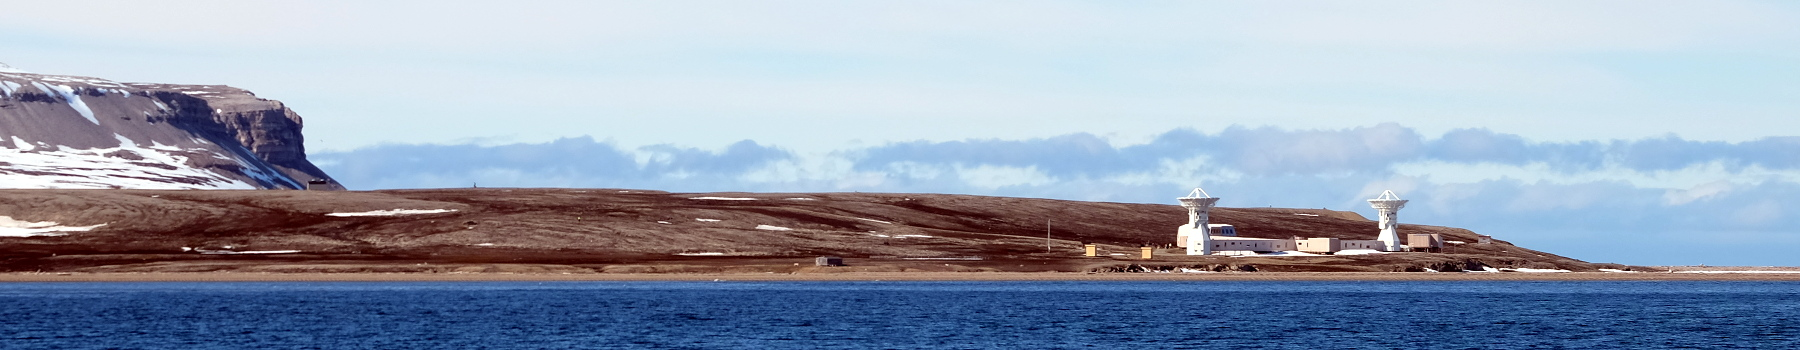
\includegraphics[width=.8\paperwidth]{figure/brandal2}
      
    The Norwegian Mapping Authority is building a new observatory at Ny-Ålesund ...
  \end{centering}
  \pause

  \begin{itemize}
  \item<2-> We want more control over the data Ny-Ålesund delivers than we currently have
  \item<3-> Because of the special working conditions, there is a high turn-over of personell at Ny-Ålesund
  \item<4-> To ensure continuity, we need expertise at the main office
  \item<5-> Distances make it hard to be as hand on as most other observatories
  \end{itemize}
\end{frame}


\begin{frame}{When?}
  \begin{centering}
    A short history of the Where project:
  \end{centering}
  \pause

  \begin{itemize}
  \item<2-> NMA took over the Geosat software and tried to adapt it for geodetic analysis
  \item<3-> We attempted to contribute to ITRF2014, but had to give up due to issues with the code
  \item<4-> Based on experiences with Geosat, we started development on Where summer 2015
  \end{itemize}

  \only<5->{
  Some features of Where:
  \begin{itemize}
  \item Support for all conventional models
  \item Can do VLBI analysis, and some SLR and GNSS analyses
  \item Estimation using a Kalman filter
  \end{itemize}}
\end{frame}


\begin{frame}{Who?}

  The Where team consists of four researchers at the NMA:
  
\begin{columns}[c]
    \column{0.24\textwidth}
    \begin{center}
      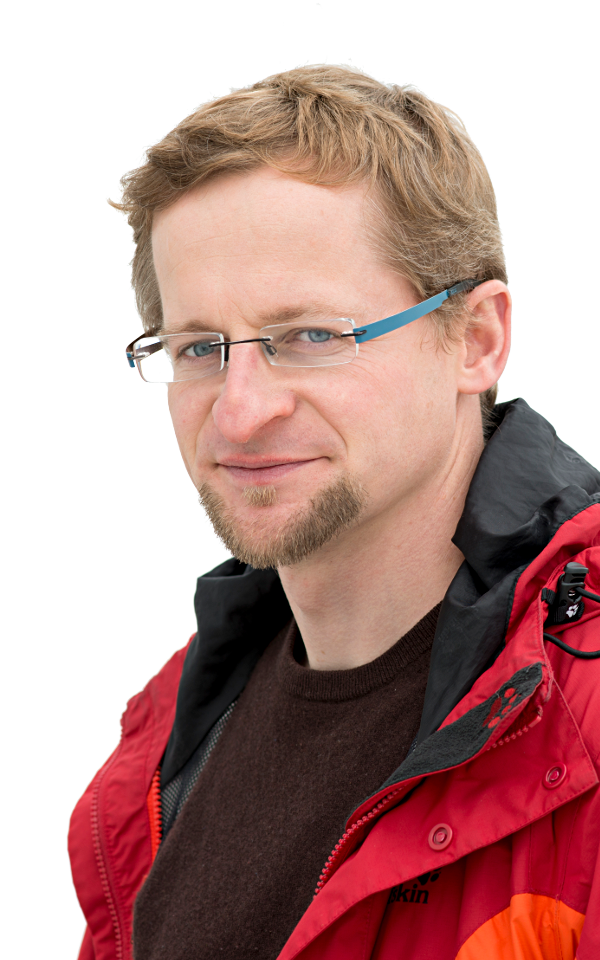
\includegraphics[width=\linewidth]{figure/michael} \\
      Michael Dähnn
    \end{center}

    \column{0.24\textwidth}
    \begin{center}
      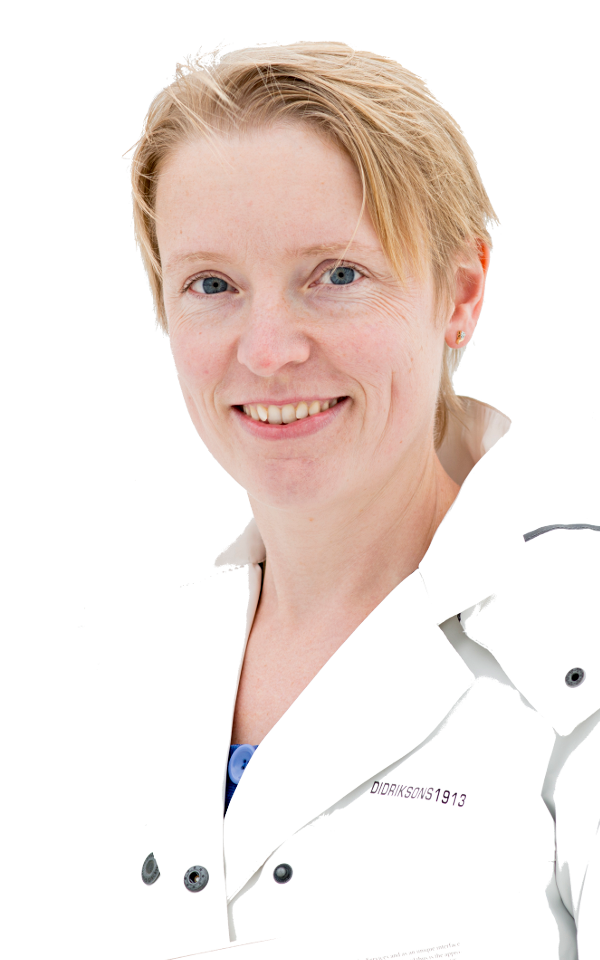
\includegraphics[width=\linewidth]{figure/ingrid} \\
      Ingrid Fausk
    \end{center}

    \column{0.24\textwidth}
    \begin{center}
      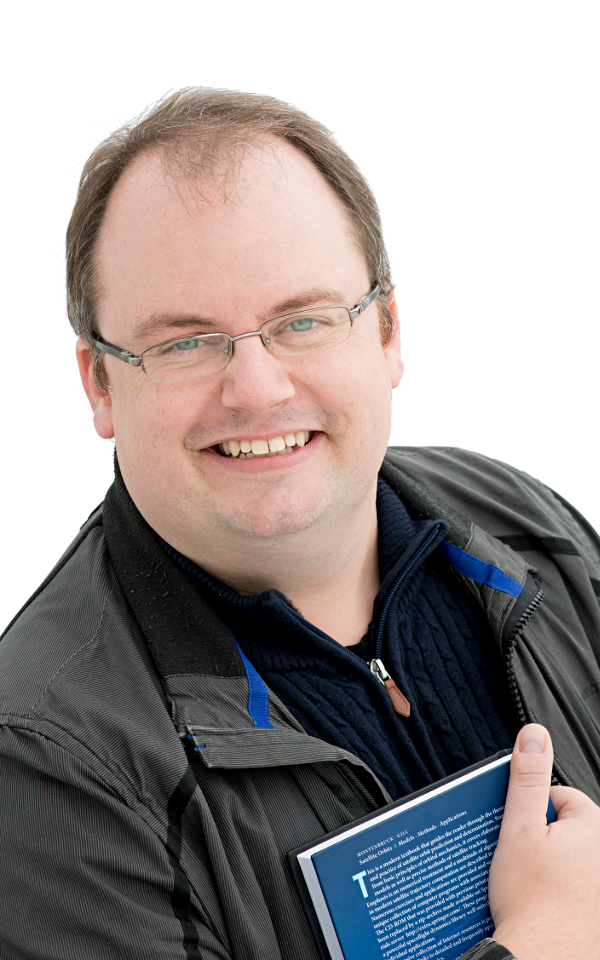
\includegraphics[width=\linewidth]{figure/geirarne} \\
      Geir Arne Hjelle
    \end{center}

    \column{0.24\textwidth}
    \begin{center}
      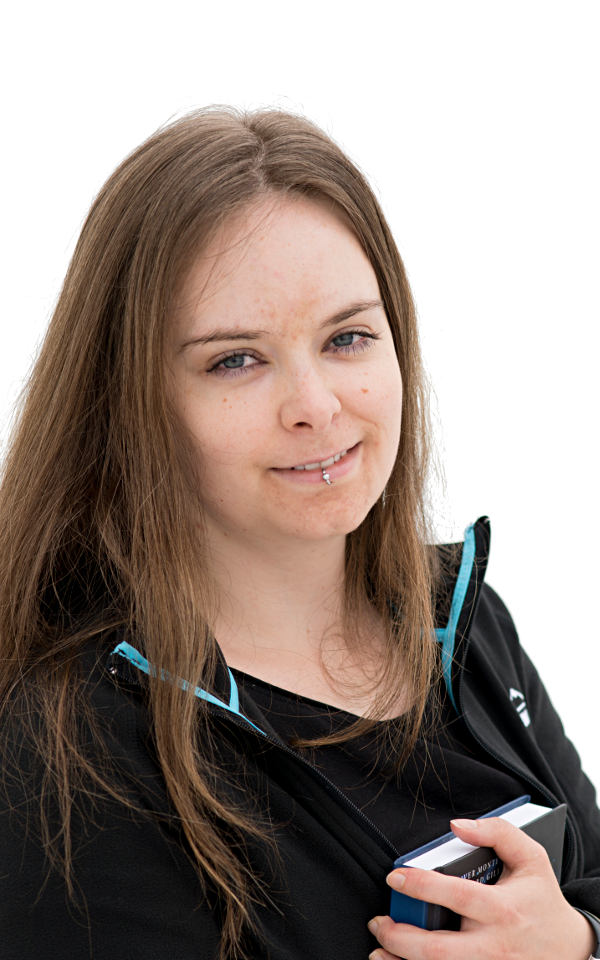
\includegraphics[width=\linewidth]{figure/annsilje} \\
      \small{Ann-Silje Kirkvik}
    \end{center}
  \end{columns}
\end{frame}


\begin{frame}{What?}
  \begin{centering}
    Where is a Python program, taking advantage of the modern Python data science stack
  \end{centering}
  \pause

  \begin{itemize}
   \item Modular code: Easy to add new models, different versions of model etc
   \item Available free and cross platform
   \item No dependencies on legacy softwares
  \end{itemize}
  \pause

  \begin{itemize}
  \item At the moment, the VLBI module is available
  \item Work on the SLR and GNSS modules are ongoing
  \end{itemize}
\end{frame}


\begin{frame}{What?}
  \begin{columns}
    \begin{column}[T]{0.49\textwidth}
      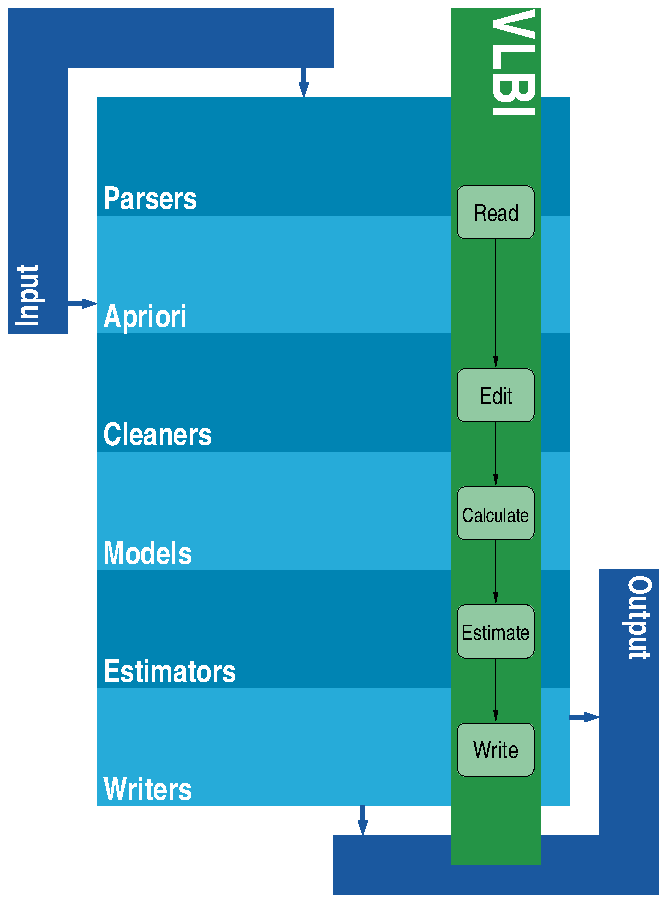
\includegraphics[width=\textwidth]{figure/code_structure_vlbi}
    \end{column}

    \begin{column}[T]{0.49\textwidth}
      Each analysis in Where is defined as a pipeline:
      \pause
    
      \begin{itemize}
      \item Data are stored at each stage
      \item Different analyses use different pipelines
      \item Different pipelines may use the same apriori data, models, estimators etc
      \end{itemize}
    \end{column}
  \end{columns}
\end{frame}


\begin{frame}{What?}
  \begin{centering}
    NMA has been an Associate Analysis Center with the IVS for several years.
  \end{centering}
  \pause

  \begin{itemize}
  \item We aim to become an operational analysis center
  \item We are submitting solutions to the IVS Combination Center
  \end{itemize}

  \includegraphics[width=0.75\paperwidth]<3>{figure/NYALES20-E_diff-trf}
  \includegraphics[width=0.75\paperwidth]<4>{figure/NYALES20-N_diff-trf}
  \includegraphics[width=0.75\paperwidth]<5>{figure/NYALES20-H_diff-trf}
  \includegraphics[width=0.7\paperwidth]<6>{figure/dut_nma_diff_combi}
  \includegraphics[width=0.7\paperwidth]<7>{figure/lod_nma_diff_combi}
  \includegraphics[width=0.7\paperwidth]<8>{figure/x-pole_nma_diff_combi}
  \includegraphics[width=0.7\paperwidth]<9>{figure/x-pole-rate_nma_diff_combi}
\end{frame}


\begin{frame}[fragile]{What?}

  \begin{centering}
    The VLBI Analysis Software Comparison Campaign (VASCC) [Klopotek 2016]
  \end{centering}
  \pause
  
  \begin{itemize}
  \item We participated in VASCC in the fall of 2015 with Geosat (which confirmed the issues we had been seeing in the
    spring)
  \item We redid the VASCC analysis, comparing the theoretical delay of Where with VieVS and C5++
  \end{itemize}
  \pause

  The results of this mini-VASCC were presented at EVGA 2017:
  \renewcommand{\arraystretch}{1.1}
  \begin{tabularx}{\columnwidth}{lrCCC}
  &       & \multicolumn{3}{c}{RMS [mm] Northern}   \\ \cline{3-5}
  &       & \textbf{Where}  & \textbf{c5++}   & \textbf{VieVS}  \\
  \multirow{3}{*}{\rotatebox[origin=c]{90}{Southern}}
    & \multicolumn{1}{|l}{\textbf{Where}} & $\diamond$ &     $0.49$ &     $0.44$ \\
    & \multicolumn{1}{|l}{\textbf{c5++}}  &     $0.18$ & $\diamond$ &     $0.21$ \\
    & \multicolumn{1}{|l}{\textbf{VieVS}} &     $0.43$ &     $0.39$ & $\diamond$ \\
  \end{tabularx}
\end{frame}

\begin{frame}{How?}
  \begin{centering}
    We are making Where available for the VLBI community!
  \end{centering}
  \pause
  
  \begin{itemize}
  \item<2-> MIT Open Source License: Permissive, use Where as you want
  \item<3-> But please acknowledge us if you use Where :)
  \item<4-> Also: Do get in touch if you are interested in Where. We'd love to help you get started, and hear about your experiences.
  \end{itemize}
\end{frame}


\begin{frame}{Where!}

  Version 0.8.1 of Where is now available at
  \begin{itemize}
  \item https://github.com/kartverket/where
  \end{itemize}
  \pause

  The version number is still < 1.0:
  \begin{itemize}
  \item As noted, we are still seeing a few issues
  \item We will reimplement the internal time series data structure
  \item Our plan is to release version 1.0 this year
  \item The current version only includes the VLBI pipeline
  \end{itemize}

\end{frame}


\begin{frame}{Where to?}

  \begin{centering}
    Some of the things we are working on at the moment:
  \end{centering}
  \pause
  
  \begin{itemize}
  \item<2-> Main focus: Finish application as IVS analysis center
  \item<3-> Set up infrastructure for delivering operational analysis
  \item<4-> Cooperation with Yebes/IGN, also on analysis software
  \item<5-> A paper about Where is to be submitted to the Journal of Open Source Software
  \item<6-> Implement least squares estimation and compare with Kalman filter
  \item<7-> Simplified installation and better Windows support
  \end{itemize}
\end{frame}


\begin{frame}[c]{Thank you!}
  \LARGE https://github.com/kartverket/where
\end{frame}
  

\end{document}
